\documentclass{beamer}

% importations de packages utiles
\usepackage[utf8]{inputenc}  % pouvoir écrire avec des accents
\usepackage[french]{babel}  % francophopnie
\usepackage{hyperref}  % liens clicables dans pdf final
\usepackage{tikz}  % pouvoir tracer des dessins sympas
\usetheme{Boadilla}  % thème de beamer
\usepackage{listingsutf8}  % rendu de "code" (avec config ci-dessous)
\definecolor{lstcolor}{rgb}{0.9,0.95,0.95}
\definecolor{lstcommentcolor}{rgb}{0.,0.2,0.}
\lstset{
  frameround=tttt,
  %autogobble,
  frame=single,
  backgroundcolor=\color{lstcolor},
  % extendedchars=true,
  % basicstyle=\ttfamily\small,
  keywordstyle=\bfseries\color{blue},
  identifierstyle=\bfseries\color{red},
  stringstyle=\bfseries\color{orange},
  commentstyle=\color{lstcommentcolor},
  language=Python,
  keepspaces=True,
  basicstyle=\fontfamily{pcr}\selectfont\small, % monospace it for copypasting
  upquote=true,
  columns=flexible,
  showstringspaces=False,
  literate={é}{{\'e}}1
}
\title{La Concurrence}
\subtitle{Concepts de Langages de Programmation}
\author{Juan-Carlos Barros et Daniel Kessler}
% et c'est parti
\begin{document}
\begin{frame}
  \titlepage
\end{frame}

\begin{frame}
  \tableofcontents
\end{frame}

\section{Introduction}
\begin{frame}
  \frametitle{Introduction: la concurrence en-dehors de l'informatique}
  \begin{itemize}
  \item Définition
  \item Cerveau vs CPU
  \item L'OS
  \end{itemize}
\end{frame}
\begin{frame}
  \frametitle{Définition} La \textbf{programmation concurrente} est une forme de
  programmation dans laquelle plusieurs tâches sont exécutées simultanément
  (pendant des périodes qui se chevauchent) au lieu de séquentiellement (l’une
  démarrant après la fin de l’autre).
\end{frame}
\begin{frame}
  \frametitle{La concurrence est en nous}
  Le \tetxbf{cerveau} est intrisèquement \textbf{concurrent}.
  \begin{minipage}{.5\linewidth}
    \begin{itemize}
    \item traitement du stimulus visuel
    \item traitement du stimulus auditif
    \item traitement de la syntaxe, grammaire puis sémantique
    \item analyse du sens
    \item comparaison avec les connaissances mémorisées
    \item critique
    \end{itemize}
  \end{minipage}
  \begin{minipage}{.5\linewidth}
    \LARGE
    \vfill
    Ce mot est \color{green}{rouge}.
    \vfill
    Ce mot est \color{blue}{vert}.
    \vfill
    Ce mot est \color{red}{bleu}.
    \vfill
  \end{minipage}
\end{frame}
\begin{frame}
  \frametitle{La séquence est dans l'ordinateur}
  Le \textbf{processeur} est intrinsèquement \textbf{séquentiel}.
  \begin{minipage}{.5\linewidth}
    \begin{itemize}
    \item Une instruction exécutée à la fois
    \item Pourquoi chercher la concurrence?
      \begin{itemize}
      \item Interruptions I/O
      \item Exécuter plusieurs programmes ``simultanément''
      \item Systèmes distribués
      \end{itemize}
    \end{itemize}
  \end{minipage}
  \begin{minipage}{.5\linewidth}
    IMAGE PAS EXPORTABLE DU WYSIWYG JCB
  \end{minipage}
\end{frame}
\begin{frame}
  \frametitle{OS: le maître de la concurrence}
  Le \textbf{système d'exploitation} est un ``magicien''.
  \begin{minipage}{.5\linewidth}
    \begin{itemize}
    \item gestion des ressources séquentielles
    \item couche d'abstraction
    \item partage des ressources:\par
      $\rightarrow$ \textbf{l'ordonnanceur}
      \begin{itemize}
      \item gestion des priorités
      \item commutation des contextes
      \item gestion des dangers de la concurrence
      \end{itemize}
    \end{itemize}
  \end{minipage}
  \begin{minipage}{.5\linewidth}
    IMAGE PAS EXPORTABLE DU WYSIWYG JCB    
  \end{minipage}
\end{frame}

\section{Les fondamentaux de la concurrence}
\begin{frame}
  \frametitle{Les foncdamentaux de la concurrence}
  Comment se manifeste la concurrence?
  \begin{itemize}
  \item multplicité des machines
  \item multiplicité des processeurs
  \item multiplicité des \textbf{processus}
  \item multiplicité des \textbf{fils d'exécution} (threads)
  \end{itemize}

  Comment communiquent les différents composants?
  \begin{itemize}
  \item de manière \textbf{synchrone}: contact direct
  \item de manière \textbf{asynchrone}: message envoyé, arrivera plus tard
  \item via des \textbf{ressources communes}: source de problème
    \par$\rightarrow$\textbf{sections critiques}
  \end{itemize}
\end{frame} % la concurrence, comment?
\begin{frame}
  \frametitle{Problèmes et solutions}
  \begin{minipage}{.5\linewidth}
    Problèmes
    \begin{itemize}
    \item Situation de compétition
    \item Inversion de priorité
    \item Entrelacement
    \item Interblocage
    \item Famine
    \item etc.
    \end{itemize}
  \end{minipage}
  \begin{minipage}{.5\linewidth}
    Solutions
    \begin{itemize}
    \item Verrous
    \item Atomicité
    \item Moniteurs
    \item Sémaphores
    \item Futures, Promises
    \item Autres paradigmes
    \end{itemize}
  \end{minipage}
\end{frame} % problèmes et solutions
\begin{frame} 
  \frametitle{Problème 1: la \textbf{Race Condition}}
  \begin{minipage}{.5\linewidth}
    \begin{itemize}
    \item Exemple 1 (Java): corruption de données pour un compteur partagé par
      deux tâches concurrentes
    \item Exemple 2 (débranché): \ldots
    \end{itemize}
  \end{minipage}
  \begin{minipage}{.5\linewidth}
    IMAGE PAS EXPORTABLE DU WYSIWIG JCB
  \end{minipage}
\end{frame} % race condition
\begin{frame}
  \frametitle{Solution 1: le \textbf{verrou} (lock)}
  Un \textbf{verrou} limite l'accès d'une ressource à une seule tâche.
  \begin{itemize}
  \item état fermé vs. état ouvert
  \item si le verrou est fermé, les tâches sont bloquées
  \item sinon, une tâche qui accède à la ressource ferme le verrou
  \item quand la tâche finit, elle ouvre le verrou
  \end{itemize}
\end{frame} % verrou
\begin{frame}
  \frametitle{Solution 2: le \textbf{sémaphore} de Dijkstra}
  \begin{minipage}{.8\linewidth}
    \begin{itemize}
    \item Inventé pour l'OS ``THE operating system''
    \item Compteur de tâches en attente de la ressource
    \item 3 primitives
      \begin{itemize}
      \item \texttt{Init(sem, max)} définit nombres d'utilisateurs max
      \item \code{P(sem)} pour accéder à la ressource
      \item \code{V(sem)} pour quitter la ressource
      \end{itemize}
    \item \texttt{P(sem)} bloque si max atteint, sinon incrémente le compteur
    \item \texttt{V(sem)} décrémente le compteur et notifie les tâches en
      attente
    \item cas particulier: \textbf{sémaphore binaire} ou \textbf{mutex} quand \texttt{max=1}.
    \end{itemize}
  \end{minipage}
  \begin{minipage}{.3\linewidth}
    IMAGE PAS EXPORTABLE DU WYSIWIG JCB
  \end{minipage}
\end{frame} % sémaphore
\begin{frame} 
  \frametitle{Solution 3: Moniteur de Hoare}
  \begin{minipage}{.5\linewidth}
    \begin{itemize}
    \item Inventé pour \textit{Equivalent Pascal} et \textit{Solo operating
        system}
    \item Verrou avec une ou plusieurs \textbf{conditions}
    \item Condition liée à \textbf{file d'attente} de processus voulant
      accéder à une ressource
    \item Équivalence avec sémaphores
    \end{itemize}
  \begin{minipage}{.5\linewidth}
    \onslide<1>{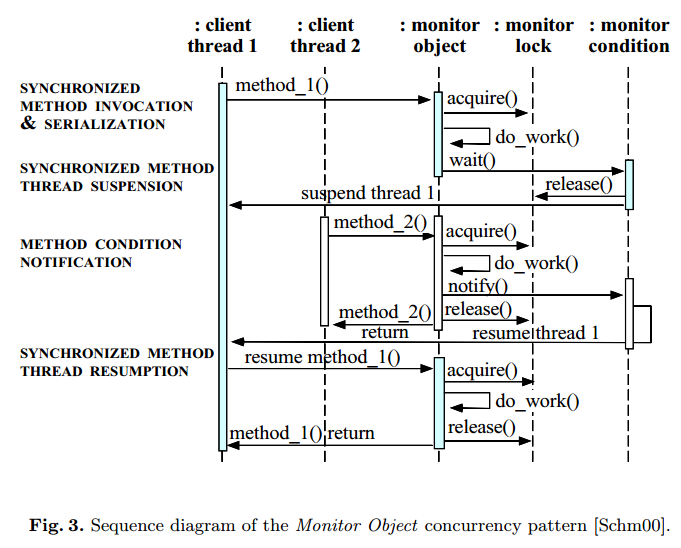
\includegraphics[width=.5\linewidth]{monitor.png}}
    \onslide<2>{\begin{lstlisting}[language=Java]
      public class SynchronizedCounter {
        private int c = 0;

        public synchronized void increment() {
          c++;
        }

        public synchronized void decrement() {
          c--;
        }

        public synchronized int value() {
          return c;
        }
      }
    \end{lstlisting}
    \hfill\textit{exemple Java}}
  \end{minipage}
  \end{minipage}
\end{frame} % moniteur

\section{Modèle d'Acteurs de Hewitt}
\begin{frame}
  \frametitle{Éviter la mémoire partagée?}
  \begin{itemize}
  \item La mémoire partagée est la source de la plupart des problèmes
  \item Les communications ne devraient se faire que par des \textbf{immuables}
  \end{itemize}
\end{frame}
\begin{frame}[fragile]
  \frametitle{Modèle d'Acteurs de Hewitt}
  Un \textbf{acteur} peut:
  \begin{itemize}
  \item Envoyer des \textbf{messages} à d'autres acteurs
  \item Créer d'autres acteurs
  \item Décider de son comportement à la prochaine réception de message
  \end{itemize}
\end{frame}
\begin{frame}[fragile]
  \frametitle{Modèle d'Acteurs de Hewitt}
  Le langage \textbf{Erlang} exploite bien ce modèle.
  \begin{center}
\begin{lstlisting}[language=erlang]
-module(acteur).
-export([start/0, machin/0]).

machin() ->
    receive
        hello ->
            io:format("Machin dit bonjour.~n", [])
    end.

start() ->
    Machin_PID = spawn(acteur, machin, []),
    Machin_PID ! hello.
\end{lstlisting}
\end{center}
  Plus récemment, le langage \textbf{Scala} utilise ce même modèle, à travers le
  ``toolkit'' \textbf{Akka}.
\end{frame}
\begin{frame}
  \frametitle{Modèle d'Acteurs de Hewitt}
  Le modèle d'acteurs a influencé le \textbf{$\pi$-calculus} (algèbre de processus)
  \par\bigskip
  \begin{quotation}\small
    Now, the pure $\lambda$-calculus is built with just two kinds of thing: terms
    and variables. Can we achieve the same economy for a process calculus? Carl
    Hewitt, with his actors model, responded to this challenge long ago; he
    declared that a value, an operator on values, and a process should all be
    the same kind of thing: an actor.

    (\ldots)
    
    So, in the spirit of Hewitt, our first step is to demand that all things
    denoted by terms or accessed by names—values, registers, operators,
    processes, objects—are all of the same kind of thing; they should all be
    processes.
  \end{quotation}
  \hfill Robin Milner, inventeur du $\pi$-calculus (\textit{Turing Lecture} 1993)
\end{frame}
\begin{frame}[fragile]
  \frametitle{Modèle d'Acteurs de Hewitt}
  Lauer et Needham on montré en 1978 que les modèles de concurrence basé sur
  processus et les modèles basés sur messages sont équivalents (``duaux'').
  \par\bigskip
  \hfill{$\rightarrow$ \footnotesize{}cf. \textit{On the duality of operating system structures}
    H. Lauer, R. Needham 1978}
\end{frame}

\section{Autres approches}
\begin{frame}
  \frametitle{Autres approches}
  \begin{itemize}
  \item{Programmation événementielle} 
  \begin{itemize}
  \item utile pour les GUIs, mais difficile à analyser
  \item ``event loop''
  \item ``event handlers'' (callbacks)
  \end{itemize}
  
  \item{Transactions }
  \begin{itemize}
  \item idée inspirée des Bases de Donnée
  \item rendre ``atomique'' la section critique
  \item idée exploitée par exemple dans le langage \textbf{Clojure}
  \end{itemize}
  
  \item{Coroutines}
  \begin{itemize}
  \item coroutines: des routines concurrentes pouvant ``vivre'' dans le même thread
  \item idée exploitée par exemple dans le langage \textbf{Go} (``goroutines'')
  \end{itemize}

  \item{Réseaux de Petri} (pour la modélisation)
  \end{itemize}
\end{frame}

\section{Conclusion}
\begin{frame}
  \frametitle{Conclusion: au-delà de la concurrence}
  Réseaux de neurone!
\end{frame}


\end{document}